\subsection*{Basics of Relations}
\begin{defn}[Relations]\index{relation}\index{Cartesian product}\index{subset}
    A \emph{relation} between to sets \(A\) and \(B\) is a subset of their Cartesian product \(A\times B\).  For example given \(A=\left\{1,3,5,7,9\right\}\) and \(B=\left\{2,3,5,7\right\}\),
    \[L=\left\{(1,2),(1,3),(1,5),(1,7),(2,3),(2,5),(2,7),(3,5),(3,7),(5,7)\right\}\]
    is a relation between \(A\) and \(B\).  We normally prefer to describe the relation, for example we can describe \(L\) by \[\forall x\in A\, \forall y\in B: x\, L\, y\ \text{if and only if}\ x<y,\]
    or equivalently \[L=\left\{(x,y)\middle|x\in A\wedge y\in B\wedge (x<y)\right\}.\]
\end{defn}

\begin{practiceprob}
    Let \(E=\left\{2n\middle|n\in\bbN\right\}\) and \(O=\left\{2n+1\middle|n\in\bbN\right\}\).  Define a relation by 
        \[\forall x\in E\, \forall y\in O: x\, D\, y\ \text{if and only if}\ x=2y.\]
    List five additional ordered pairs in the relation \(D\):
    {\large
        \[D=\left\{(2,1),(14,7),(26,13),\hspace{240pt}\right\}\]
    }

    Write the set of ordered pairs for \(D\) in set builder notation: \vspace{4\baselineskip}
\end{practiceprob}

\begin{practiceprob}
    Define a relation on the set \(\bbZ\) by 
    \begin{equation}\label{rel:mod5}
        M_5=\left\{(x,y)\middle|x,y\in\bbZ \wedge \exists q\in\bbZ: x-y=5q\right\}
    \end{equation}
    List five additional ordered pairs in the relation \(M_5\):
    {\large
        \[M_5=\left\{(17,12),(30,5),(-20,-45),\hspace{240pt}\right\}\]
    }
    Write the a description of \(M_5\) using quantifiers: \vspace{4\baselineskip}
\end{practiceprob}

\clearpage

\subsection*{Properties of Relations}
% reflexive, symmetric, transitive, antisymmetric
\begin{defn}[Properties of Relations]\index{relation! properties}\index{reflexive}\index{symmetric}\index{transitive}\index{antisymmetric}
\index{relation!reflexive}\index{relation!symmetric}\index{relation!transitive}\index{relation!antisymmetric}
    Of special interest are relations between a set and its self, such as \(M_5\) described in equation (\ref{rel:mod5}).  In particular when we have a relation \(R\) between a set \(A\) and its self we look for the following properties:
    \begin{enumerate}
        \item \emph{Reflexive:} \(\forall a\in A: a\,R\, a\),
        \item \emph{Symmetric:} \(\forall a,b\in A:\) if \(a\,R\, b\), then \(b\, R\, a\),
        \item \emph{Transitive:} \(\forall a,b,c\in A:\) if \(a\,R\, b\) and \(b\,R\, c,\)  then \(a\, R\, c\), and
        \item \emph{Antisymmetric:} \(\forall a,b\in A:\) if \(a\,R\, b\) and \(b\,R\,a\), then \(a=b\).
    \end{enumerate}

    Recall that in equation (\ref{rel:mod5}) a pair of integers \((x,y)\) were in the relation \(M_5\) if and only if their difference, \(x-y\), was a multiple of 5.  For example \((17,12)\in M_5\) since \(17-12=5\), similarly \((12,-28)\in M_5\) since \(12-(-28)=40=8\times 5\).  But we can note that:
    \begin{align}
        (12-17)&=-1\times(17-12)\nonumber\\
            &= -1\times 5 \label{eq:symmetry_M5_1},\\
        (-28-12)&=-1\times(12-(-28))\nonumber\\
            &=-8\times 5\label{eq:symmetry_M5_2},\ \text{and}\\
        (17-(-28))&=(17-12)+(12-(-28))\nonumber\\
            &=5+8\times 5\nonumber\\
            &=9\times5\label{eq:transitive_M5}.
    \end{align}
    Therefore we get that \((12,17), (-28,-12)\), and \((17,-28)\) are in \(M_5\) as well.  
    
    Further, the calculations in equations (\ref{eq:symmetry_M5_1}) and (\ref{eq:symmetry_M5_2}) can be generalized to show that {\em if \((a,b)\in M_5\), then \((b,a)\in M_5\)}, i.e. \(M_5\) is a \emph{symmetric} relation.  
    
    The calculation in equation (\ref{eq:transitive_M5}) can likewise be generalized to show that {\em if \((a,b)\) and \((b,c)\) are in \(M_5\), then \((a,c)\) is also in \(M_5\)}, i.e. \(M_5\) is a \emph{transitive} relation.  
    
    Finally, since
    \begin{equation}\label{eq:reflexive_M5}
        n-n=0=0\times 5
    \end{equation}
    for all integers \(n\), we know that {\em for all integers \(n\), \((n,n)\) is in \(M_5\)}, i.e. \(M_5\) is \emph{reflexive}.

    Since, \(M_5\) is reflexive, symmetric, and transitive we say that it is an \emph{equivalence relation}.
    \index{relation!equivalence relation}\index{equivalence relation}

    If a relation is reflexive, {\em antisymmetric}, and transitive, like the less than or equal to relation, then we say it is a \emph{partial-ordering}.\index{partial-ordering}\index{relation!partial-ordering}
\end{defn}

\clearpage

\begin{practiceprob}
    Consider the relation \(M_7\) defined by:
    \begin{equation*}
        \forall x,y\in\bbZ: x\, M_7\,y\ \text{if and only if}\ \exists q\in\bbZ: (x-y)=7q.
    \end{equation*}
    Rewrite \(M_7\) in set builder notation and list five ordered pairs of integers in \(M_7\).  Then try to show that \(M_7\) is reflexive, symmetric and transitive, i.e. it is an equivalence relation.
    \vspace{0.3\textheight}
\end{practiceprob}\index{relation!reflexive}\index{relation!symmetric}\index{relation!transitive}\index{relation!equivalence relation}

\begin{practiceprob}
    Consider the relation \(L\) defined by:
    \begin{equation*}
        \forall x,y\in\bbZ: x\, L\, y\ \text{if and only if}\ x< y
    \end{equation*}
    Rewrite \(L\) in set builder notation and list five ordered pairs of integers in \(L\).  Try to show that \(L\) is antisymmetric and transitive, then give examples showing that it is not reflexive or symmetric and so is not an equivalence relation.
    \vspace{0.3\textheight}
\end{practiceprob}

\clearpage

\begin{practiceprob}
    Consider the relation \(L^\prime\) defined by:
    \begin{equation*}
        \forall x,y\in\bbZ: x\, L^\prime\, y\ \text{if and only if}\ x\leq y
    \end{equation*}
    Rewrite \(L^\prime\) in set builder notation and list five ordered pairs of integers in \(L^\prime\). (Try to list some that were not in \(L\).)  Try to show that \(L^\prime\) is reflexive, antisymmetric, and transitive, then give examples showing that it is not symmetric and so is not an equivalence relation.  Relations like \(L^\prime\) are called \emph{partial-ordering}.
    \vspace{0.3\textheight}
\end{practiceprob}\index{relation!partial-ordering}

\begin{practiceprob}
    Consider the relation \(D\) defined by:
    \begin{equation*}
        \forall x,y\in\bbZ: x\, D\, y\ \text{if and only if}\ x=2y
    \end{equation*}
    Rewrite \(D\) in set builder notation and list five ordered pairs of integers in \(D\).  Try to show that \(D\) is antisymmetric, then give examples showing that it is not reflexive, symmetric, or transitive and so is not an equivalence relation.
    \vspace{0.3\textheight}
\end{practiceprob}

\clearpage

\begin{practiceprob}
    Consider the relation \(B_\epsilon\) defined by:
    \begin{equation*}
        \forall x,y\in\bbR: x\, B_\epsilon\, y\ \text{if and only if}\ |x-y|<\epsilon
    \end{equation*}
    Rewrite \(B_\epsilon\) in set builder notation and list five ordered pairs of real number in \(B_\epsilon\) in the case when \(\epsilon=0.5\), i.e. \(B_{0.5}\).  Try to show that \(B_{0.5}\) is reflexive and symmetric, then give examples showing that it is not transitive and so is not an equivalence relation.
    \vspace{0.3\textheight}
\end{practiceprob}

\begin{practiceprob}\label{prob:rational_rel}
    Consider the relation \(Q\) defined by:
    \begin{equation*}
        \forall x,y\in\bbR: x\, Q\, y\ \text{if and only if}\ x-y\in\bbQ
    \end{equation*}
    Rewrite \(Q\) in set builder notation and list five ordered pairs of real number in \(Q\).  Try to show that \(Q\) is an equivalence relation.
    \vspace{0.3\textheight}
\end{practiceprob}

\clearpage

\begin{practiceprob}
    Consider the relation \(W\) defined by:
    \begin{quote}
        Two words, \(x\) and \(y\), are in \(W\) if and only if they begin and end with the same letters
    \end{quote}
    For example \((their,tear)\in W\), but \((there,tear)\not\in W\).  Try to write \(W\) in set builder notation and list five ordered pairs of words in \(W\) and five pairs not in \(W\).  Try to show that \(W\) is reflexive, symmetric, and transitive, i.e. that it is an equivalence relation.
    \vspace{0.3\textheight}
\end{practiceprob}

\clearpage

\subsection*{Visualizing Relations}

\begin{exposition}{Subset Relation}
    Given a set \(X=\{a,b,c\}\) we can define a partial-ordering on \(\mathscr{P}(X)\) using the subset or equal to relation:
        \[A\sim B\ \text{if and only if}\ A\subseteq B.\]
    We can then visualize this as a graph where all the subsets are vertices and two vertices are connected if there is a relation between them.

    \begin{figure}[H]
    \centering
    \begin{subfigure}{0.45\textwidth}
        \centering
        % \inputtikz{setrelationdiagram}
        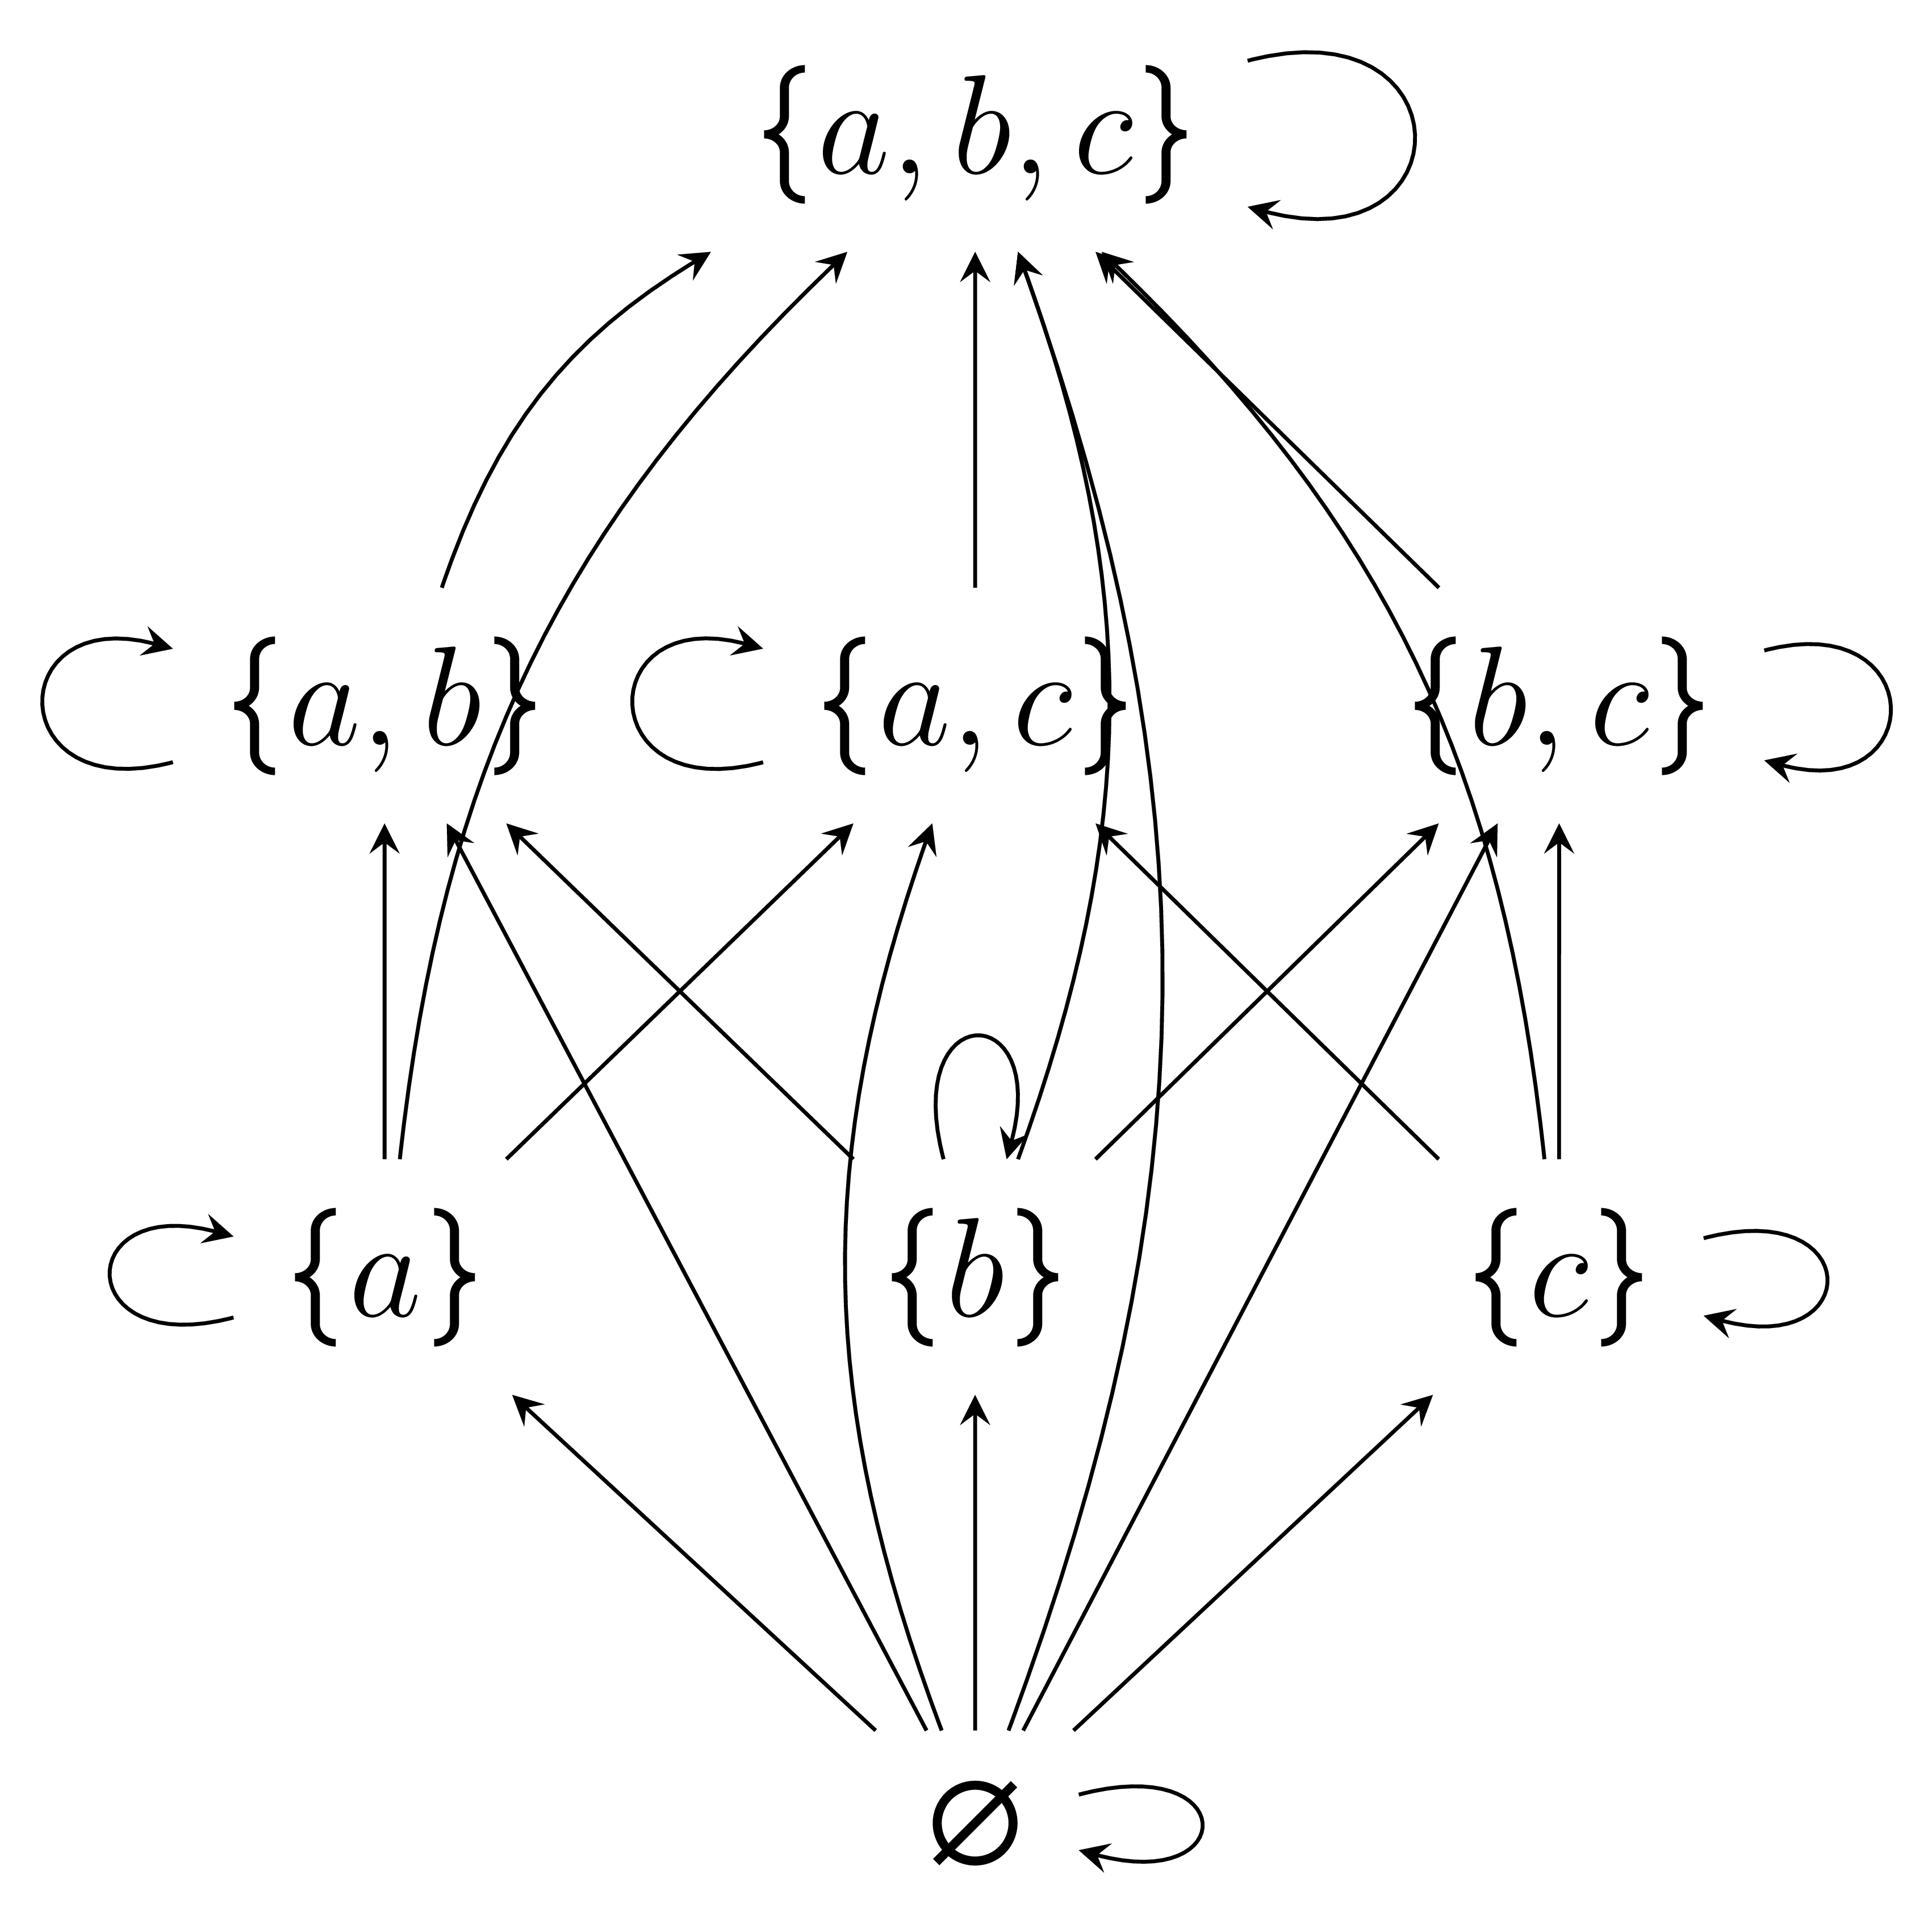
\includegraphics[scale=0.24,alt={subset relation mapped out as a graph}]{images/created/setrelationdiagram.png}
        \caption{Diagram of Subset Relation}
        \label{fig:subsetrelation}        
    \end{subfigure}
    \begin{subfigure}{0.45\textwidth}
        \centering
        % \inputtikz{setrelationhassediagram}
        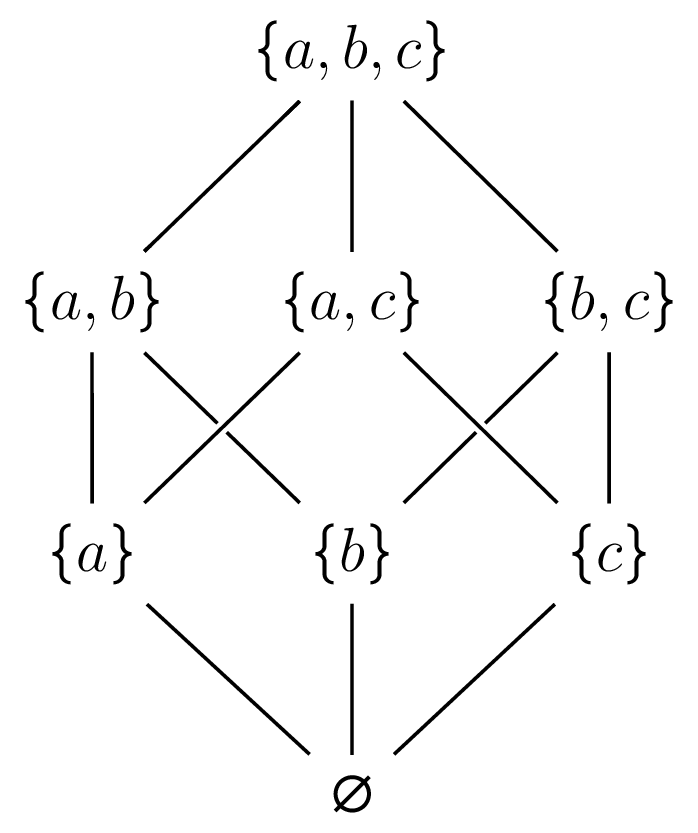
\includegraphics[scale=0.24,alt=subset relation mapped out as a hasse diagram]{images/created/setrelationhassediagram.png}
        \caption{Hasse Diagram of Subset Relation}
        \label{fig:hassesubsetrelation}        
    \end{subfigure}
    \end{figure}

    In the first diagram each time an element \(x\) relates to an element \(y\) we draw an arrow from \(x\) to \(y\).  The second diagram is drawn assuming we have a partial-ordering and the physically lowest value in the diagram is the \emph{minimal value} in the partial-ordering, the loops are implied, and so are arrows going from lower values to higher.

\end{exposition}

\begin{practiceprob} Looking at the graph of a relation on the right:
\begin{sides}[lefthand width=0.6\textwidth]
    \begin{enumerate}
        \item How do we know this relation is {\em reflexive}?\vspace{\baselineskip}
        \item How do we know this relation is {\em symmetric}?\vspace{\baselineskip}
        \item How do we know this relation is not {\em transitive}?\vspace{\baselineskip}
    \end{enumerate}
    \tcblower
        \centering
        % \inputtikz{relationgraph_1}
        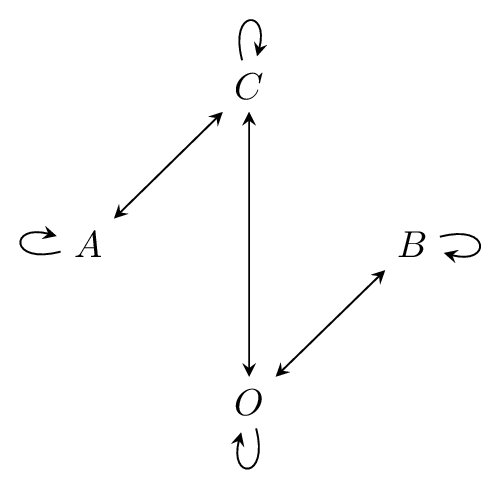
\includegraphics[scale=0.24,alt={graph of a reflexive and symmetric relation}]{images/created/relationgraph_1.png}
\end{sides}    
\end{practiceprob}

\clearpage

\begin{practiceprob} Looking at the graph of a relation on the right:
\begin{sides}[lefthand width=0.6\textwidth]
\begin{enumerate}
    \item How do we know this relation is {\em reflexive}?\vspace{\baselineskip}
    \item How do we know this relation is {\em antisymmetric}?\vspace{\baselineskip}
    \item How do we know this relation is {\em transitive}?\vspace{\baselineskip}
\end{enumerate}
\tcblower
        \centering
        % \inputtikz{relationgraph_2}
        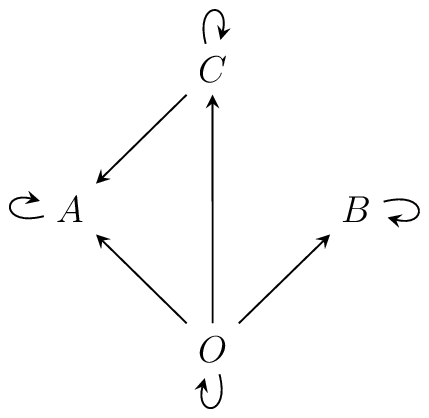
\includegraphics[scale=0.24,alt={graph of a partial ordering},width=0.7\linewidth]{images/created/relationgraph_2.png}
\end{sides}
\end{practiceprob}

\begin{practiceprob} Looking at the graph of a relation on the right:
\begin{sides}[lefthand width=0.6\textwidth]
\begin{enumerate}
    \item How do we know this relation is not {\em reflexive}?\vspace{\baselineskip}
    \item How do we know this relation is {\em symmetric}?\vspace{\baselineskip}
    \item How do we know this relation is not {\em transitive}?\vspace{\baselineskip}
\end{enumerate}
\tcblower
        \centering
        % \inputtikz{relationgraph_3}
        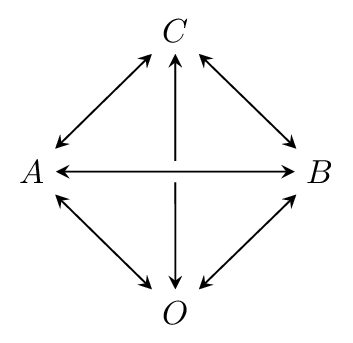
\includegraphics[scale=0.24,alt={graph of a only symmetric relation}]{images/created/relationgraph_3.png}
\end{sides}
\end{practiceprob}

\begin{practiceprob} Looking at the graph of a relation on the right:
\begin{sides}[lefthand width=0.6\textwidth]
\begin{enumerate}
    \item How do we know this relation is {\em reflexive}?\vspace{\baselineskip}
    \item Why is this relation not {\em symmetric}, {\em antisymmetric}, or {\em transitive}?\vspace{\baselineskip}
\end{enumerate}
\tcblower
        \centering
        % \inputtikz{relationgraph_4}
        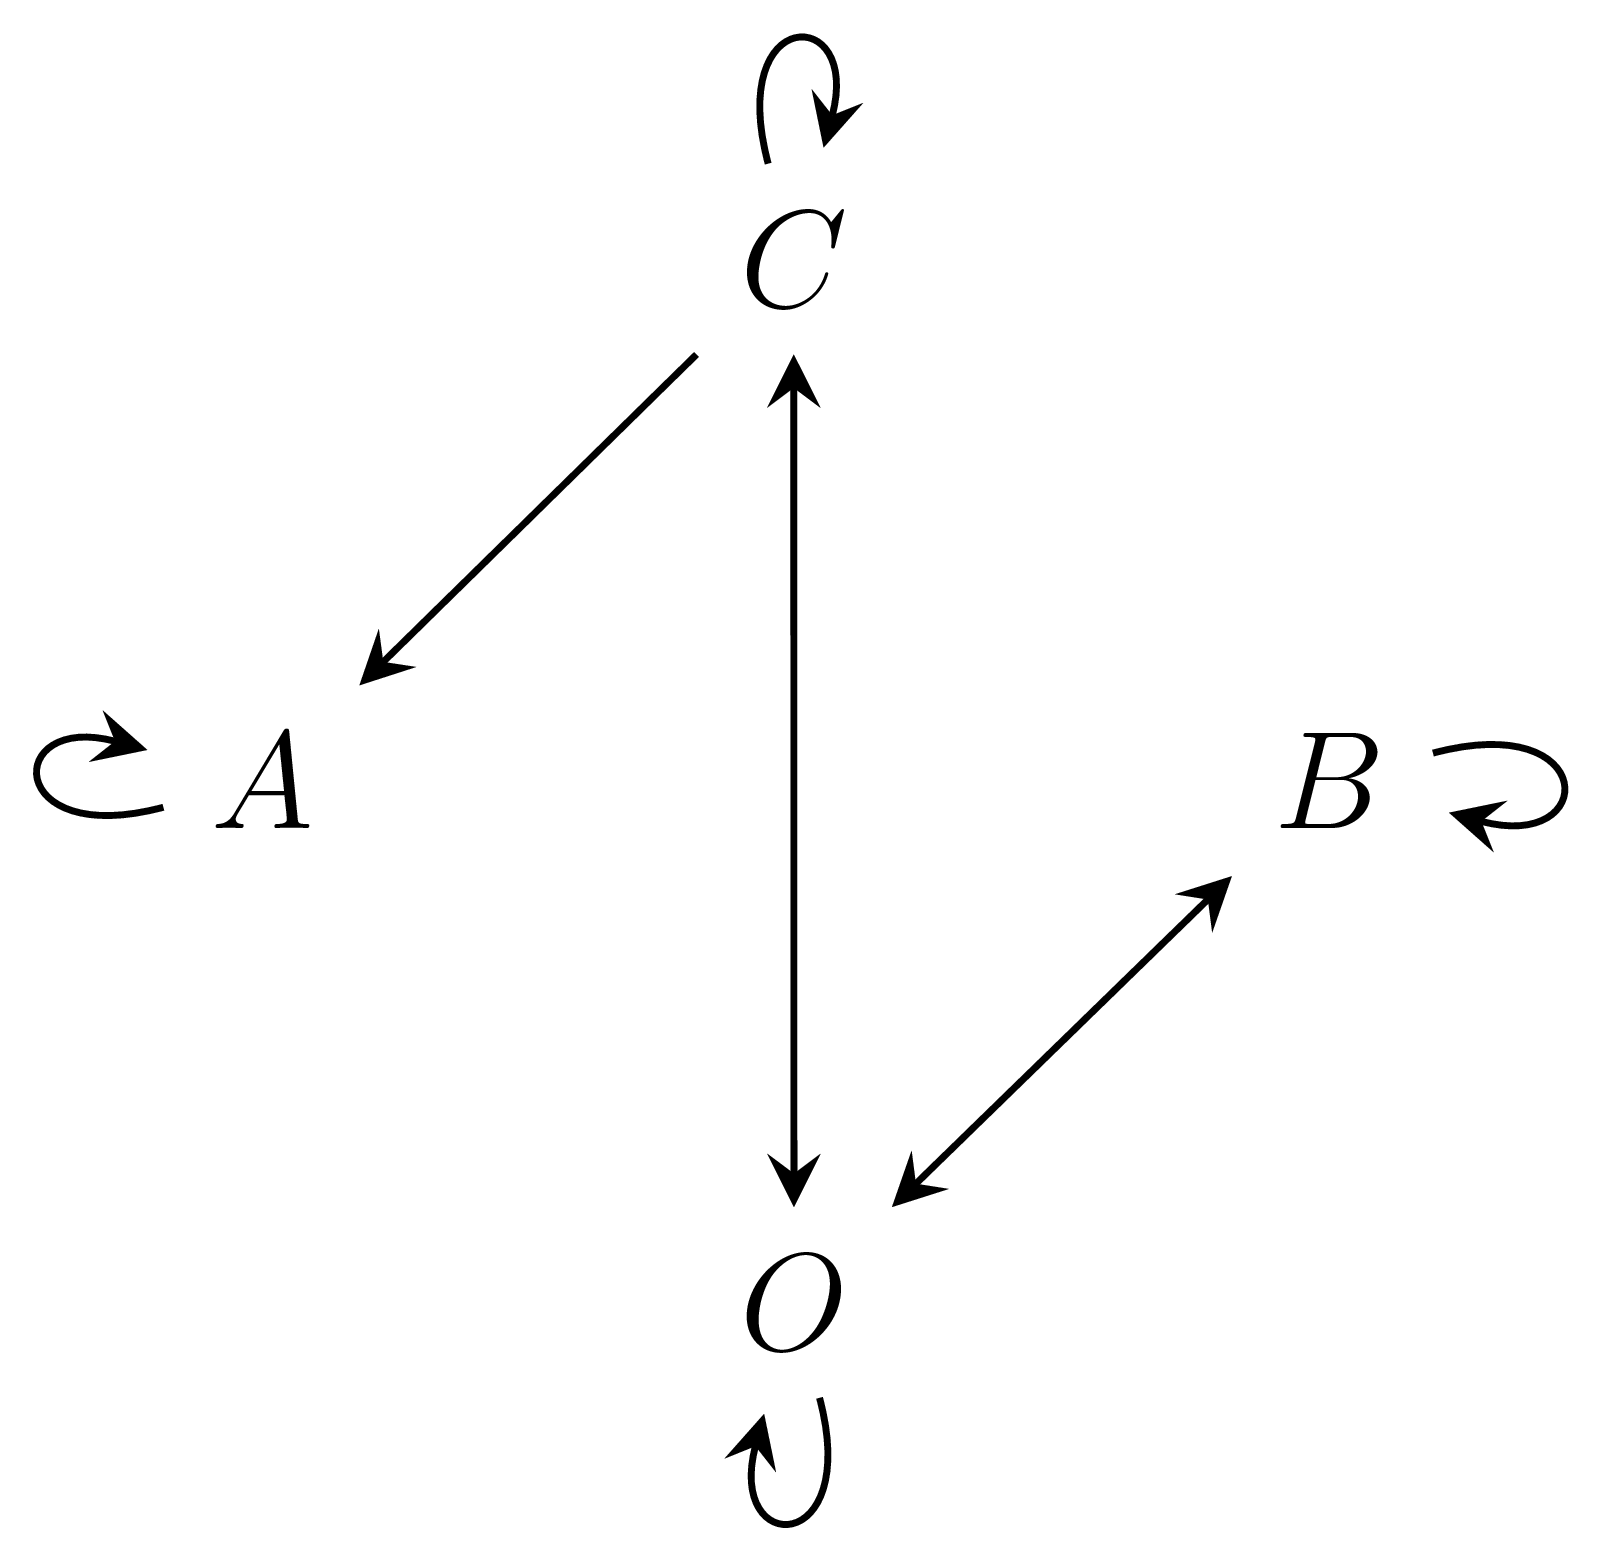
\includegraphics[scale=0.24,alt={graph of a reflexive only relation}]{images/created/relationgraph_4.png}
\end{sides}
\end{practiceprob}

\begin{practiceprob} Looking at the graph of a relation on the right:
\begin{sides}[lefthand width=0.6\textwidth]
\begin{enumerate}
    \item How do we know this relation is {\em reflexive}?\vspace{\baselineskip}
    \item Why is this relation {\em symmetric}, {\em antisymmetric}, and {\em transitive}?\vspace{\baselineskip}
\end{enumerate}
\tcblower
        \centering
        % \inputtikz{relationgraph_5}
        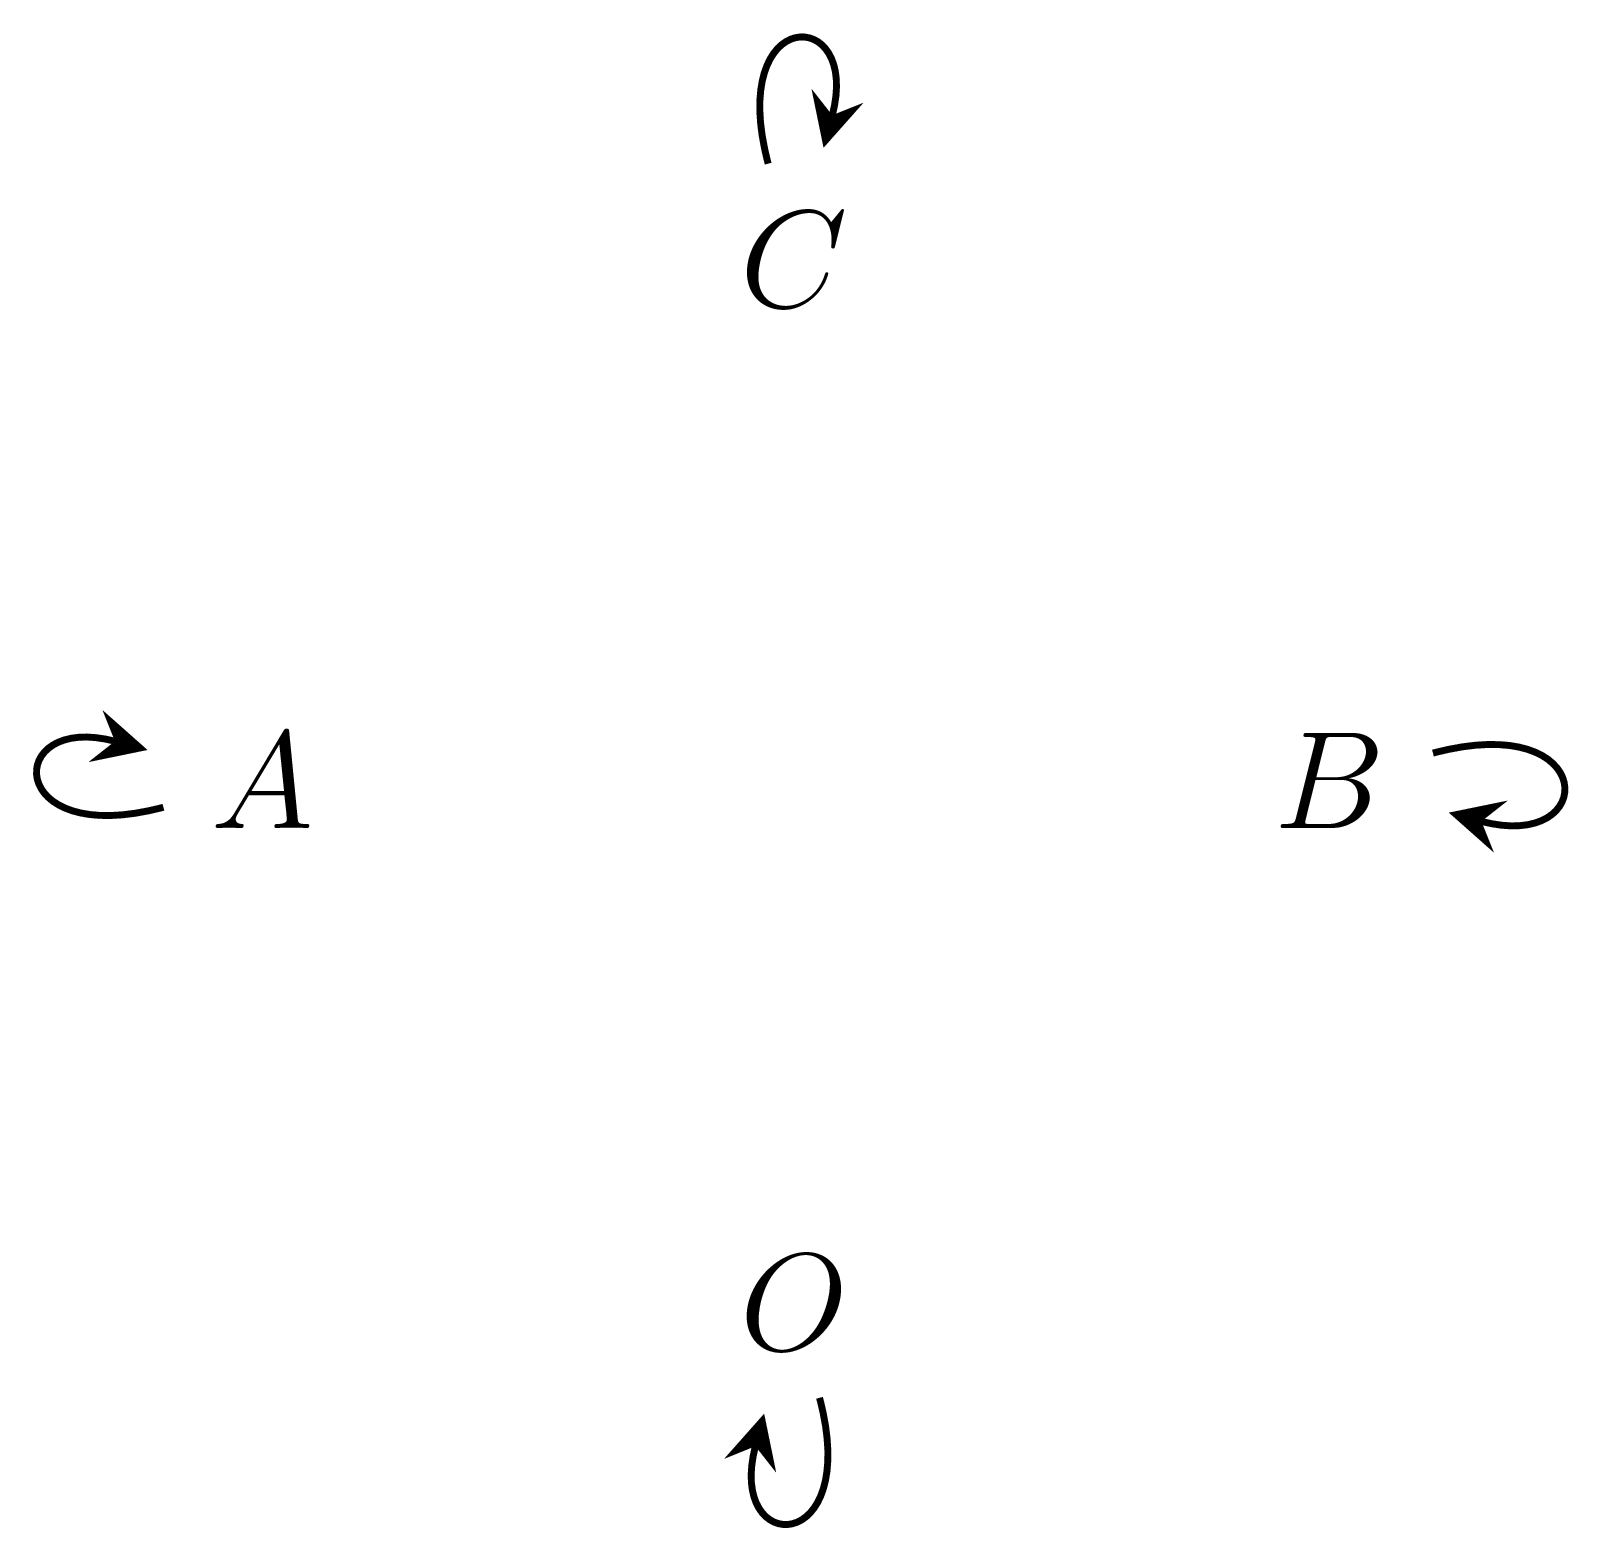
\includegraphics[scale=0.24,alt={graph of a trivial equivalence relation}]{images/created/relationgraph_5.png}
\end{sides}
\end{practiceprob}


\clearpage

\subsection*{Equivalence Classes}

\begin{exposition}\index{equivalence class}\index{equivalence relation}\index{equivalence class representative}
    Earlier we saw that the relation \(M_5\) (equation (\ref{rel:mod5}) p.\pageref{rel:mod5}) was an equivalence relation, i.e. it is reflexive, symmetric, and transitive. We also saw that the values 17, 12, and -28 are all \emph{``equivalent''}.  If we group all the integers together which are equivalent using \(M_5\) we get five sets:
    \begin{itemize}
        \item \([0]=\left\{0,\pm5,\pm10,\pm15,\ldots\right\}
            =\left\{5k\middle| k\in\bbZ\right\}\)
        \item \([1]=\left\{1,6,-4,11,-9,16,-14,\ldots\right\}
            =\left\{1+5k\middle| k\in\bbZ\right\}\)
        \item \([2]=\left\{2,7,-3,12,-8,17,-13,\ldots\right\}
            =\left\{2+5k\middle| k\in\bbZ\right\}\)
        \item \([3]=\left\{3,8,-2,13,-7,18,-12,\ldots\right\}
            =\left\{3+5k\middle| k\in\bbZ\right\}\)
        \item \([4]=\left\{4,9,-1,14,-6,19,-11,\ldots\right\}
            =\left\{4+5k\middle| k\in\bbZ\right\}\)
    \end{itemize}
    And, because of the symmetry and transitivity of the relation \([n]\cap[m]=\emptyset\) whenever \(n\neq m\).  We call these sets \emph{equivalence classes} and the values 0, 1, 2, 3, and 4 are \emph{equivalence class representatives}, we let them stand in for all the numbers they are equal to.
\end{exposition}

\begin{defn}[Equivalence Class]
    Given an equivalence relation \(\mathcal{R}\) defined on a set \(S\) we say that two elements of \(a,b\in S\) are in the same \emph{equivalence class} of \(\mathcal{R}\) if and only if \(a\) is related to \(b\) by \(\mathcal{R}\), \(a\mathcal{R} b\).  Alternately, we can say that the equivalence class for \(a\) is the set of all \(b\) such that \(a\mathcal{R}b\), which is written:
        \[[a]_{\mathcal{R}} = \left\{b\in S\middle|a\mathcal{R}b\right\}\]
    If \(a\) is the element of the equivalence class we typically work with we call it the \emph{equivalence class representative}.  Further, we can show that: 
    \begin{itemize}
        \item every element of \(S\) is in exactly one equivalence class, 
        \item any two equivalence classes are either disjoint or equal, and 
        \item \(S=\bigcup_{a\in S}[a]_{\mathcal{R}}\).
    \end{itemize}
    These three conditions give us a \emph{partition} of \(S\).\index{partition}

    \begin{figure}[H]
        \centering
        % \inputtikz{partition_of_Z}
        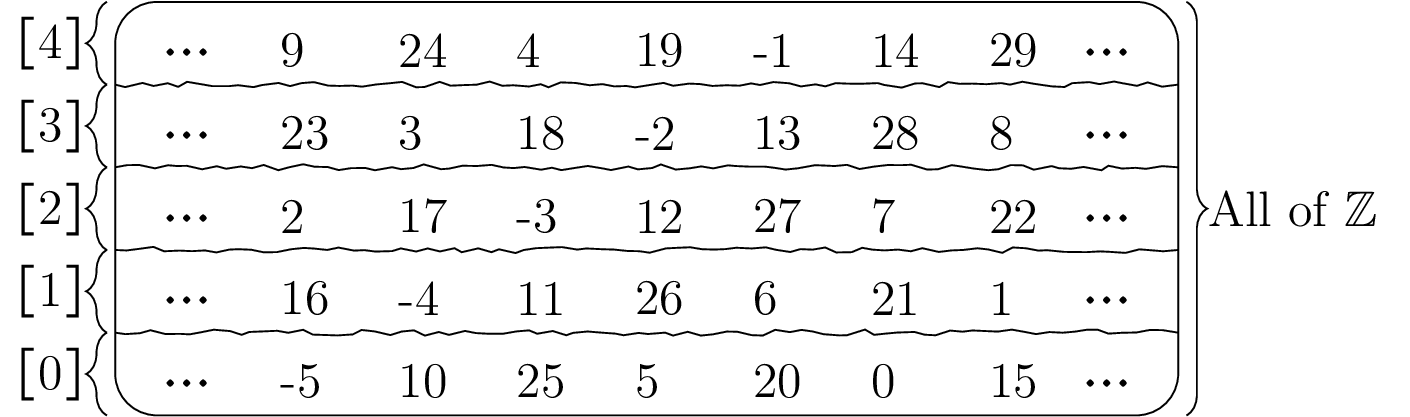
\includegraphics[scale=0.24,alt={the set of integers partitioned by the relation mod 5}]{images/created/partition_of_Z.png}
        \caption{Relation \(M_5\) Partitioning \(\bbZ\)}
        \label{fig:Mod5Partition}
    \end{figure}
    
\end{defn}

\begin{practiceprob}
    Earlier we defined the relation \(M_7\) as:
    \begin{equation*}
        \forall x,y\in\bbZ: x\, M_7\,y\ \text{if and only if}\ \exists q\in\bbZ: (x-y)=7q.
    \end{equation*}
    We then {\em``showed''} that it was an equivalence relation.  This relation will have seven equivalence classes with representatives 0, 1, 2, 3, 4, 5, and 6.  Try to write down/describe the elements of the equivalence classes:
    \begin{itemize}
        \foreach \i in {0,...,6}{
            \item \([\i]=\left\{\phantom{\rule{0.3\textwidth}{15pt}}\right\}
            =\left\{\phantom{\rule{0.24\textwidth}{15pt}}\middle|\phantom{\rule{0.15\textwidth}{15pt}}\right\}\)
        }
    \end{itemize}    
\end{practiceprob}

\begin{practiceprob}\index{modular equivalence}
    The relations \(M_5\) and \(M_7\) are specific examples of \emph{equivalence modulo \(n\)}:
    \begin{equation}\label{eq:modequiv}
        \forall x,y\in\bbZ: x\equiv y\pmod{n}\ \text{if and only if}\ \exists q\in\bbZ: (x-y)=qn.
    \end{equation}
    As with \(M_5\) and \(M_7\) this defines and equivalence relation.  This relation will have \(n\) equivalence classes with representatives \(0\leq k\leq (n-1)\).  Try to write down/describe the elements of a general equivalence class:
    \begin{align}
        [k]&=\left\{\phantom{\rule{0.6\textwidth}{25pt}}\right\}\\
            &=\left\{\phantom{\rule{0.34\textwidth}{25pt}}\middle|\phantom{\rule{0.25\textwidth}{15pt}}\right\}
    \end{align}
    The idea of equivalence modulo \(n\) plays an important role in many areas of Math and Computer Science. Modular calculations are built into most programming languages with commands such as \verb|%, mod, fmod, rem|, and  \verb|remainder|.
\end{practiceprob}

\clearpage

\begin{practiceprob}
    Earlier in Problem \ref{prob:rational_rel} on page \pageref{prob:rational_rel}, we said \(x\) and \(y\) are related by \(Q\) if and only if \(x-y\in\bbQ\) and showed that it was an equivalence relation.  List five distinct equivalence classes in \(Q\).
    \begin{itemize}
        \item \(C_1\) = \vspace{2\baselineskip}
        \item \(C_2\) = \vspace{2\baselineskip}
        \item \(C_3\) = \vspace{2\baselineskip}
        \item \(C_4\) = \vspace{2\baselineskip}
        \item \(C_5\) = \vspace{2\baselineskip}
    \end{itemize}
    Do you think it is possible to list all the equivalence classes for this relation? Why or Why Not?
    \vspace{10\baselineskip}
\end{practiceprob}

\clearpage

\begin{practiceprob}
The graph represents an, admittedly boring, equivalence relation.  What are the four equivalence classes?

% \inputtikz{eq_class_diagram}
    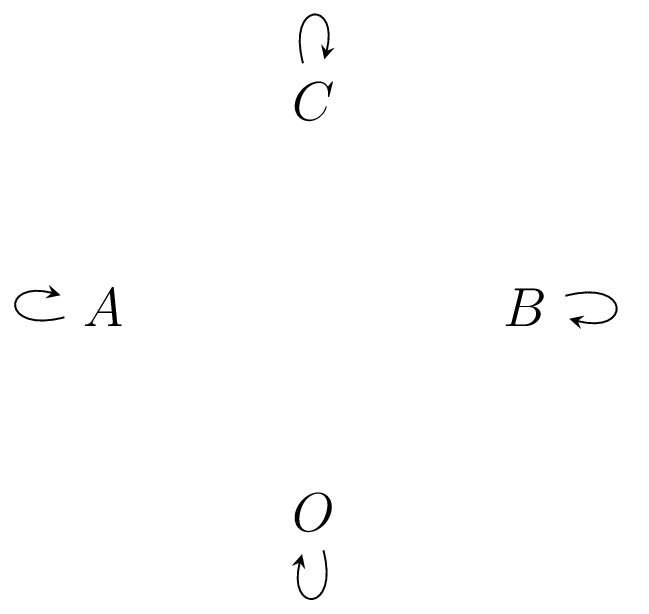
\includegraphics[scale=0.24,alt={graph of an equivalence relation with four singleton equivalence classes}]{images/created/eq_class_diagram.png}
\end{practiceprob}

\begin{practiceprob}
The graph represents an equivalence relation.  Why is there only one equivalence class?

% \inputtikz{eq_class_diagram2}
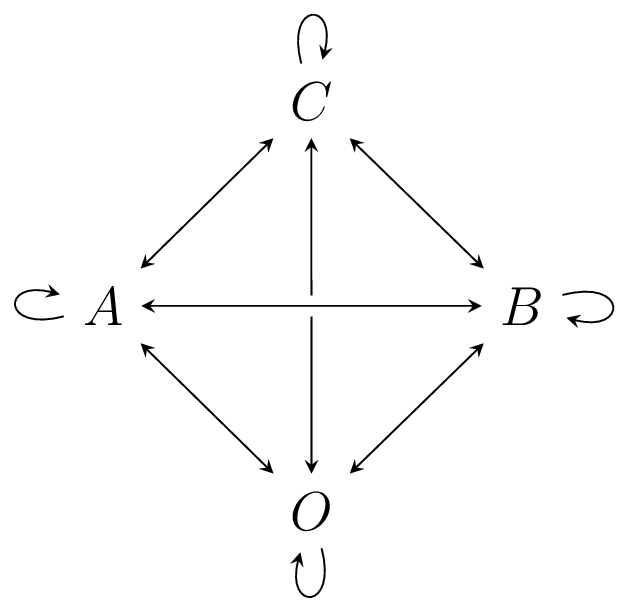
\includegraphics[scale=0.24,alt={graph of an equivalence relation with one equivalence class}]{images/created/eq_class_diagram2.png}
\end{practiceprob}

\begin{practiceprob}
The graph represents an equivalence relation.  What are the equivalence classes?

% \inputtikz{eq_class_diagram3}
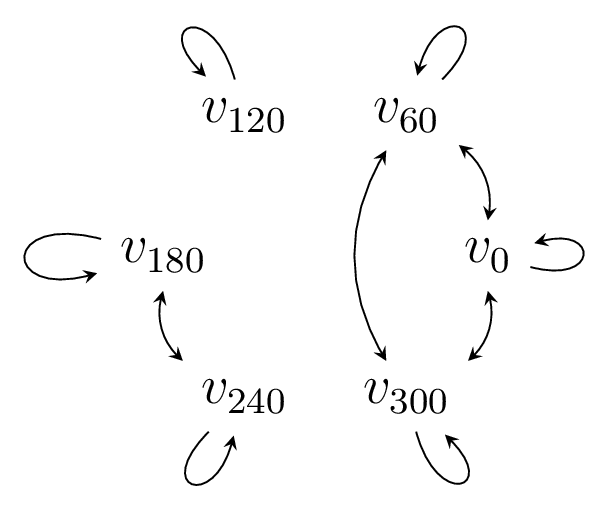
\includegraphics[scale=0.24,alt={graph of an equivalence relation with three equivalence classes}]{images/created/eq_class_diagram3.png}
\end{practiceprob}
